\chapter{Electromagnetism}
\section{Intro}
Electrical circuits are fundamental building blocks in, more or less, every electronic device you can think of. The simple act of flipping a switch, e.g. to turn on the light, completes an electrical circuit. The purpose of the circuit is to carry electrical current, either in an open or closed circuit. The electrical components in a circuit are typically resistors, capacitors,  switches, and an electrical 	source (a battery, for instance).
\\ 
In this chapter, if a function is assumed constant, it is denoted with capitalization of its original notation. 
\\ 
\\
A circuit is an electronic system, which consists of different elements with different functions, that change the way the circuit acts. The different elements of the circuit can be divided into two categories: active and passive. Active elements supply energy to the system, e.g. a battery, whereas passive elements absorbs energy, e.g. a light bulb. A circuit with a battery and a bulb can be represented in the following way. 
\begin{figure}
	\begin{center}
	\begin{circuitikz}[american voltages]
	\draw 
		(0,0) to[battery, battery1=$V_{battery}$] (0,2)
		to[lamp, l=$Lightbulb$] (2, 2)
		to[short] (2,0)
		to[resistor, R=$R$] (0,0);
		
	\end{circuitikz}
\end{center}
\end{figure}
\\ This circuit consist of an active element, a battery, and a passive element, a light bulb. Charge is transported by the current from the positive terminal of the battery, through to the light bulb. The light bulb absorbs the energy from the charge, which is then transported to the negative terminal of the battery.
\\
\section{Current}
Current is the force that moves charge through a circuit. Current can be defined as an amount of charge moved over a time interval. This can be expressed as the following relation:
\begin{align}
i(t)=\dfrac{dq(t)}{dt} \Leftrightarrow q(t)=\int_{-\infty}^{t}i(x)dx
\end{align}
where $i(t)$ is the current (in ampere $A$), to a given time $t$ (in seconds $s$), and $q(t)$ is the function for charge at a given time $t$. $q(t)$ is measured in Coulomb$(C)$.
\\
There exists two types of current, Alternating Current (AC) and Direct current (DC). DC current is constant, while AC alternates, see figure. WHAT FIGURE? REFERENCE
\\
\section{Voltage}
Voltage ($V$), also called electric potential difference, is the change of potential energy a charge undergoes when it passes through two given points in a circuit. This is expressed in the following equation:
\begin{align}
	V=\dfrac{dU(q)}{dq}
\end{align}
\\
where $U(q)$ (in joules $J$) is the function for potential energy, given a charge $q$.
\section{Resistor}
When a resistor, which is a passive element, is added to the circuit it creates a resistance ($\Omega$). Resistance makes it more difficult for the current to pass through the element. Resistance is defined as the proportional constant between current and voltage, the mathematical relation of this is given by:
\begin{align} 
\label{Ohm}
v(t)=R\cdot i(t),  R\geq0
\end{align}
where $R$ is resistance.
\section{Capacitor}
A capacitor is a passive element of a circuit. A capacitor consist of two similar sizes plates. When a voltage is applied to the circuit, the capacitor gets charged. The capacitance is the amount of energy a capacitor can store when it's fully charged. The capacitor gets charged when positive a charge is transferred from one plate, through the circuit, to the other plate. The capacitance is given by the following equation:
\begin{align*}
C=\dfrac{\epsilon_{0}A}{d}
\end{align*}
where $C$ is the capacitance (in farad $F$), $\epsilon_{0}$ is the permittivity of free space which is equal to $8.85 \cdot 10^{-12}                                                 \frac{F}{m}$. $A$ is the surface area of the plates (in square meters $(m^{2})$), and $d$ is the distance between the two plates (in meters $m$).
\\
The charge of a capacitor across a voltage ($V$) and capacitance of ($C$) is equal to:
\begin{align}
\label{QCV}
Q=CV	
\end{align}

\textbf{Time constant}
\\
The time constant ($\tau$) is defined as.
\begin{align}
\tau = RC
\end{align}
Even though the graph for (??) have a horizontal asymptote, the capacitor is defined as fully charged at $5\tau$.

\section{Circuit diagrams}
Electrical circuits are visually represented in circuit diagrams. In addition of the above-mentioned elements, they introduce three terms: nodes, branches, and loops. A \textit{node} connects the circuit elements. These elements are also called \textit{branches}, i.e.  the voltage supply, resistors, capacitors, and the like. Lastly, is any closed path in the circuit, in which no node is encountered more than than once, called a \textit{loop} \cite[page~32]{bcircuit}. An example of a circuit is shown below.

\begin{figure}[H]
 \begin{center}
\begin{circuitikz}[american voltages]
\draw
to[battery, battery1=$V_{B}$, color=blue] (0,2)
to[resistor, R=$R_1$, color=red] (2,2)
to[resistor, R=$R_2$, color=red] (2,0)
to[short, -] (0,0)
[short, -](2,2) to [short, -] (3,2)
to[resistor, R=$R_3$, color=red](3,0)
to[short, -] (2,0)
[short](3,2) to [short] (5,2)
to [C=$C$, color=green](5,0)
to [short, -] (3,0)
(0,0) to [short, l_=$N_3$, -] (5,0)
(2,2) to [short, l^=$N_2$, -] (5,2)
(0,1) to [short, l^=$N_1$, -] (0,2);
\end{circuitikz}
\end{center}
\end{figure}

This circuit has five branches, which are shown marked in color: a battery (in blue), three resistors ($R_1, R_2,$ and $R_3$, in red), and the light bulb (in green). The three nodes of the circuit ($N_1$, $N_2$, and $N_3$) connect the branches. Additionally, there are three loops, all of which have same starting and ending point, $V_{battery}$. The first loop passes through $R_1$ and $R_2$, and returns to the starting point. Similarly, the second loop passes through $R_1$ and $R_3$, and returns. The third, and final, loop runs through $R_1$, then the light bulb, and returns. 

\subsection{Kirchhoff's Laws}
\textbf{Kirchhoff's Current Law}
\\
Observe a circuit up until a node, past which the path of the circuit splits in two. The current encountering the node does not accumulate (as it would e.g. in a battery). Instead, all electrons flowing to that node split up between the available paths, and continue to flow through the circuit. This is Kirchhoff’s current law (KCL), which states that the algebraic sum of all currents in a node is equal to zero. 
\begin{align}
\sum_{j=1}^{N} i_{j}(t) = 0
\end{align}
where $i_{j}(t)$ is the $j$'th current entering the node through branch $j$, with $N$ branches connected to the node. \cite[page~32]{bcircuit}
\\
\\
\textbf{Kirchoff's Voltage Law (KVL)}
\\
KCL states that in a circuit the algebraic sum of all currents in a loop is equal to zero. This law can be express mathematically  as.
\begin{align}
\sum_{j=1}^{N} v_{j}(t) = 0
\end{align}
where $V_{j}(t)$ is the voltage in the $k$'th loop with $N$ voltages.\citep[page~34]{bcircuit}\\

\section{RC Circuit}
An RC circuit is an electrical circuit consisting of resistors and capacitors. In its simplest form, it is composed of one of each. In that case, a charged capacitor placed in series with a resistor will discharge back through the resistor \cite[p~21]{artof}. "The voltage across the capacitor, which is time dependant, can be found using Kirchhoff's current law." (husk citation)

\begin{figure}[H]
 \begin{center}
\begin{circuitikz}[american voltages]
\draw (0,0)
to[sqV, sqV=$v_{input}$] (0,2)
to (6,2)
to[short, -] (4,2)
to[C=$C$] (4,0)
to (6,0)
to (4,0)
to [resistor, R=$R$] (0,0);
\draw [>=latex', <->] (6,1.75) -- node[anchor=west] {$v_{C}(t)$} (6,0.25);
\end{circuitikz}
\end{center}
\end{figure}

\begin{align}\label{I_C}
I_{C}= C \dfrac{dv}{dt}
\end{align}
\subsection{Transient analysis}
To find out how the voltage of a capacitor changes over time when it's charged and discharged, transient analysis is used. The function for a charging capacitor can be found as follows:
\\
According the Kirchhoff's Current Law states that the sum of the currents in a node is equal to zero. In the case of an RC-circuit, the law can be written as the following equation:
\begin{align*}
I_{C}+I_{R}=0 \Leftrightarrow 
I_{C}= -I_{R}
\end{align*}
Inserting the definition of the current through the capacitor \eqref{I_C} and the resistor \eqref{Ohm} yields a differential equation, which can then be separated as follows:
\begin{align*}
C \dfrac{dv}{dt}&=\dfrac{-V}{R} \\
\Leftrightarrow \dfrac{dv}{dt} &= \dfrac{-V}{R}\dfrac{1}{C} \\
\Leftrightarrow dv &= \dfrac{-V}{R}\dfrac{1}{C}dt \\
\Leftrightarrow \dfrac{1}{V}dv &= \dfrac{-1}{RC}dt
\end{align*}
Both sides of the equation is then integrated, and the Voltage is isolated:
\begin{align*}
\int \dfrac{1}{V}dv =& \dfrac{-1}{RC} \int dt \\
\Leftrightarrow \ln(V) =& \dfrac{-t}{RC} + A \\
\Leftrightarrow V =& e^{\frac{-t}{RC}}e^{A}
\end{align*}
Since A is the constant of integration, the constant $e^A$ can be defined as a new constant $e^A=B$.
\\
By definition the starting voltage of the capacitor is given by $V_C(t=0)=V_0$; inserting this and $B$ yields the following equation: 
\begin{align}
V(t)= e^{\frac{-t}{RC}}B \\
V(0)= B = V_0
\end{align}
The constant $B$ is then equal to start voltage $V_0$. By inserting this (3.10) in the final function is found.
\begin{align}
\label{V_down}
\Aboxed{
 V(t) = V_0e^{\frac{-t}{RC}}
 }
\end{align}
The equation \eqref{V_down} is the function, which describes how the voltage decreases over time, when the capacitor the discharged.
\\
\\
Now the function for when the capacitor charges is derived. KCL states that the sum of the voltages over a loop must be equal to zero. In an RC circuit with a battery this can be written algebraic as:
\begin{align*}
V_B-V_R-V_C =& 0 \\
\Leftrightarrow V_B=&V_R+V_C
\end{align*}
$V_R$ and $V_C$ have negative signs since their elements creates a negative potential difference when charge passes trough them.
\\
By Ohm's law \eqref{Ohm} the voltage of the resistor can be expressed as $V_R=IR$. By the definition of a capacitor \eqref{QCV} the voltage of the capacitor can be expressed as $V_C=\dfrac{Q}{C}$. This is inserted in the equation above:
\begin{align*}
V_B=&V_R+V_C \\
\Leftrightarrow \rightarrow V_B =& IR+\dfrac{Q}{C}
\end{align*}
As stated earlier current is defined as $I =\dfrac{dq}{dt}$, this is inserted in place of $I_R$. The differentials are then separated
\begin{align*}
V_B &= \dfrac{dq}{dt} R + \dfrac{Q}{C} \\
\Leftrightarrow V_B - \dfrac{Q}{C} &= \dfrac{dq}{dt}R \\
\Leftrightarrow \dfrac{1}{R}dt &= \dfrac{1}{V_B-\dfrac{q}{C}}dq \\
\Leftrightarrow \dfrac{1}{RC}dt &= \dfrac{1}{q-V_BC} dq
\end{align*}
Both side are then integrated
\begin{align*}
-\dfrac{1}{RC}\int_{0}^t dt &= \int_{0}^q \dfrac{1}{q-V_BC}dq \\
\rightarrow -\dfrac{t}{RC} &= \ln(q-V_BC) |_{0}^{q} \\
\Leftrightarrow -\dfrac{t}{RC} &= \ln(\dfrac{q-V_BC}{-V_BC}) \\
\Leftrightarrow e^{\dfrac{-t}{RC}} &= \dfrac{q-V_BC}{-V_BC} \\
\Leftrightarrow q &= V_BC(1-e^{\frac{-t}{RC}})
\end{align*}
The voltage of a capacitor is given as $V_C=\dfrac{Q}{C}$. By dividing the equation above with $C$, the function for voltage is found.
\begin{align}
\label{V_up}
\Aboxed{
V_C=V_B(1-e^{\frac{-t}{RC}})
}
\end{align}
\eqref{V_up} is the function which describes how the voltage increases over time, when the capacitor is charged.
\begin{align*}
V_R &= I \cdot R \\
V_C &= \frac{q}{C} \\
\int \frac{1}{a} &= \ln(a) \\
\ln(a) - \ln(b) &= \ln(\frac{a}{b})
\end{align*}
\\
\begin{align*}
V_B &= V_R + V_C \\
V_B &= I \cdot R + \frac{q}{C} \\
V_B &= \frac{dq}{dt} \cdot R + \frac{q}{C} \\
V_B \cdot \frac{q}{C} &= \frac{dq}{dt} \cdot R \\
(V_B - \frac{q}{C}) \cdot \frac{1}{R} &= \frac{dq}{dt} \\
\frac{1}{R} \cdot dt &= \frac{dq}{V_B - \frac{q}{C}} \\
- \frac{1}{RC} \int_{0}^{t} 1 dt &= \int_{0}^{q} \frac{1}{q-V_B C}dq \\
[-\frac{t}{RC}]_{0}^{t} &= [\ln(q-V_B C)]_{0}^{q} \\
-\frac{t}{RC} - (-\frac{0}{RC}) &= \ln(q-V_B C) - \ln(V_B C) \\
-\frac{t}{RC} &= \ln(\frac{q-V_B C}{-V_B C}) \\
e^{-\frac{t}{RC}} &= \frac{q-V_B C}{-V_B C} \\
-V_B C \cdot e^{-\frac{t}{RC}} &= q - V_B C \\
V_B C - V_B C \cdot e^{-\frac{t}{RC}} &= q \\
q(t) &= V_B C(1-e^{-\frac{t}{RC}}) \\
V_C(t) &= \frac{q(t)}{c} = V_B (1 - e^{-\frac{t}{RC}})
\end{align*}

\subsection{RC circuit experiment}
In the following section an RC circuit experiment has been made. Data from an RC circuit will be compared to values from a mathematical model. \\

\subsection{Theoretical values}
The resistance and capacitor in the experiment, had the following values:

\begin{align*}
 R =& 4770\Omega \\
 C =& 97.61nF
\end{align*}

The circuit was set up as follows:
\begin{figure}[H]
	\begin{center}
\begin{circuitikz}[american voltages]
\draw
to[sqV, sqV=$1 V$] (0,2)
to[resistor, R=$4770 \Omega$] (4.5,2)

[short](3,2) to [short] (5,2)

to [short, C=$97.61 nF$] (5,0)
(0,0) to [short, -] (5,0)

(0,1) to [short, -] (0,2);
\end{circuitikz}
\end{center}
\end{figure}
The time constant $\tau$, is then calculated $\tau = RC$. In this case $\tau$ is:
\begin{align*}
	\tau = 4.77 k\Omega \cdot 97.61 nF &= 46.56 \cdot 10^{-5} s \\
\end{align*}
Furthermore, the charging and discharging of the capacitor can then be put in a table. Since the formula $V_{charge}(t)=V_B(1-e^{\frac{-t}{RC}})$ contains $e^{\frac{-t}{RC}}$ then the table values can be calculated for different $\tau$ values. Hereby a table can be created for $V_{charge}$ and $V_{discharge}$:
\begin{table}[H]
\center
\begin{tabular}{|l|l|l|}
\hline
$\tau$ & $V_{charge}$ & $V_{decharge}$ \\ \hline
1      & 63.2\%       & 36.8\%         \\ \hline
2      & 86.5\%       & 13.5\%         \\ \hline
3      & 95.0\%       & 5.0\%          \\ \hline
4      & 98.2\%       & 1.8\%          \\ \hline
5      & 99.3\%       & 0.7\%          \\ \hline
\end{tabular}
\end{table}
Generally, the capacitor is considered fully charged, or discharged, at $5\tau$. \\
The time it takes for the capacitor to be fully charged, or discharged, is in this case:
\begin{align*}
5\tau &= 5 \cdot 46.56 \cdot 10^{-5} s \\
&= 2.33 ms
\end{align*}
\subsection{Test values comparison}
gu

\begin{figure}
\center
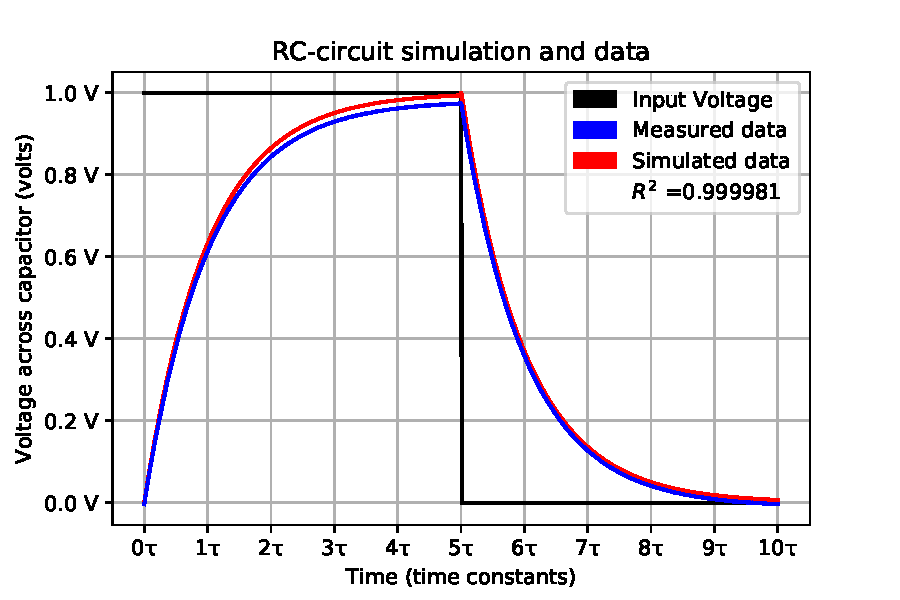
\includegraphics[scale=1]{fig/img/eks_1}
\end{figure}

\subsection{Test values comparison}
\begin{figure}[H]
 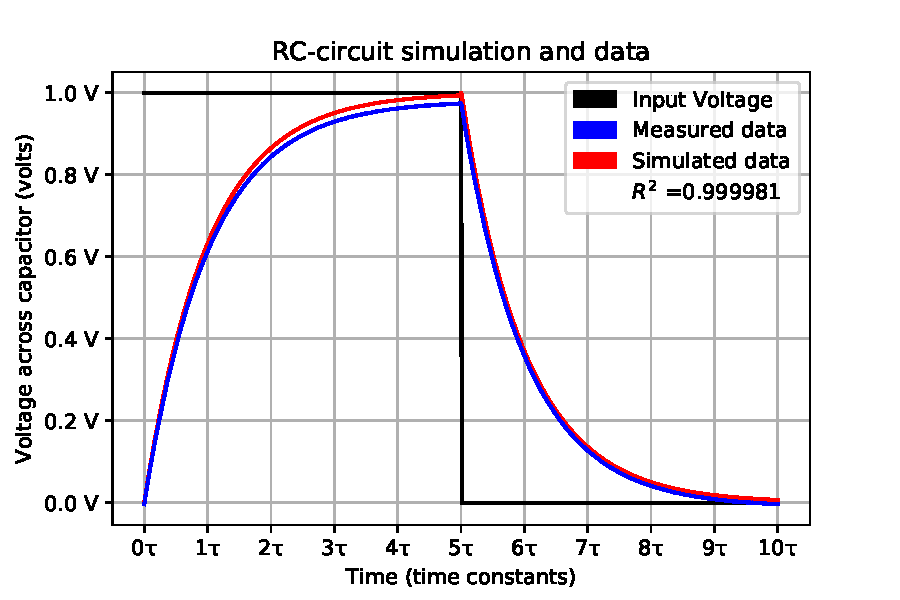
\includegraphics{fig/img/eks_1.pdf}
 \end{figure}

